%% Chapter 4: Results (chapters/chapter04.tex)

% ==============================================================================
% Chapter Writing Guidelines:
% - Presentation of data: Show raw values, processed datasets, and curves.
% - Formatting rules: Include units correctly using the siunitx package.
% - Figure rules: Captions must be located below the figure.
% - Table rules: Captions must be located above the table.
% ==============================================================================

\chapter{Results}
\label{ch:results}

This chapter details the compiled results from Z-scan experiments and validates the simulated curves.

\section{Experimental Dataset}
Table \ref{tab:material_properties} details the linear and non-linear optical properties recorded for typical calibration samples at a wavelength of $\lambda = \SI{632.8}{\nano\meter}$.

\begin{table}[H]
    \centering
    \caption{Linear and non-linear optical parameters of measured samples.}
    \label{tab:material_properties}
    \begin{tabular}{ccc}
        \toprule
        \textbf{Sample Name} & \textbf{Linear Index ($n_0$)} & \textbf{Non-linear Index ($n_2$)} \\
         & & ($\times \num{1e-16}\,\SI{}{\meter\squared\per\watt}$) \\
        \midrule
        Quartz Glass & \num{1.457} & \num{0.85} \\
        Fused Silica & \num{1.458} & \num{0.78} \\
        SF59 Glass   & \num{1.943} & \num{57.0} \\
        \bottomrule
    \end{tabular}
\end{table}

\section{Transmission Curves (pgfplots)}
Using the raw data model, we generate the normalized closed-aperture transmission profile using the \textsf{pgfplots} environment, as illustrated in Figure \ref{fig:transmission_plot}:

\begin{figure}[H]
    \centering
    \begin{subfigure}[b]{0.8\textwidth}
        \centering
        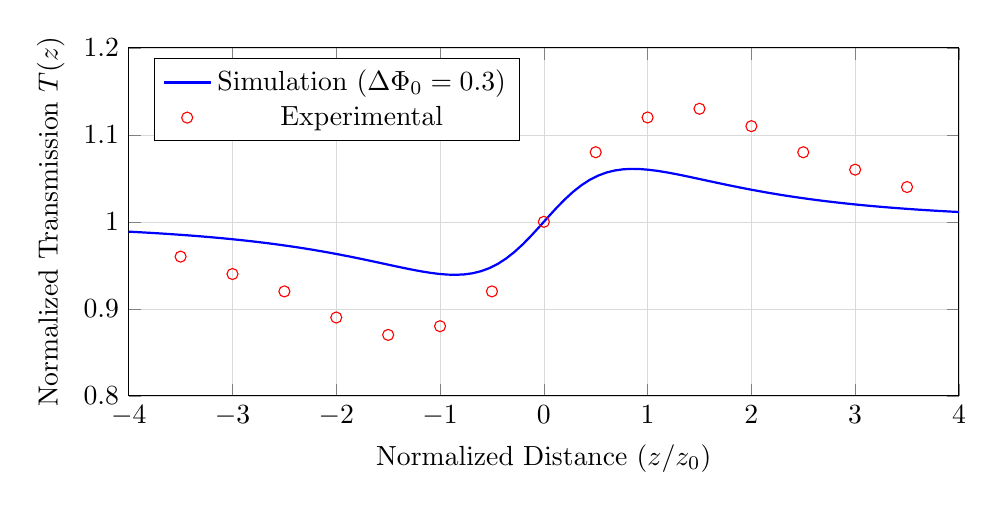
\begin{tikzpicture}
        \begin{axis}[
            width=\textwidth,
            height=6cm,
            xlabel={Normalized Distance ($z/z_0$)},
            ylabel={Normalized Transmission $T(z)$},
            xmin=-4, xmax=4,
            ymin=0.8, ymax=1.2,
            grid=both,
            grid style={line width=.1pt, color=gray!10},
            major grid style={line width=.2pt, color=gray!30},
            legend pos=north west
        ]
            % Simulated transmission curve
            \addplot[blue, thick, domain=-4:4, samples=100] 
                {1 + (4*0.3*x)/((x^2 + 9)*(x^2 + 1))};
            \addlegendentry{Simulation ($\Delta \Phi_0 = 0.3$)}
            
            % Mock experimental data points
            \addplot[red, only marks, mark=o] coordinates {
                (-3.5, 0.96) (-3.0, 0.94) (-2.5, 0.92) (-2.0, 0.89) 
                (-1.5, 0.87) (-1.0, 0.88) (-0.5, 0.92) (0.0, 1.00) 
                (0.5, 1.08) (1.0, 1.12) (1.5, 1.13) (2.0, 1.11) 
                (2.5, 1.08) (3.0, 1.06) (3.5, 1.04)
            };
            \addlegendentry{Experimental}
        \end{axis}
        \end{tikzpicture}
    \end{subfigure}
    \caption{Closed-aperture Z-scan normalized transmission curve showing peak-valley behavior.}
    \label{fig:transmission_plot}
\end{figure}
